\section{Increasing the Toy Task Complexity}\todo{titles may need changing in this section}

\section{Reaching with an Obstacle}
So, to carry this investigation to the next level I introduced an obstacle placing mechanism as well as randomly placing the target behind the obstacle. This is to ensure that the agent doesn't learn where the target can be behind a wall from where the obstacle is. See Figure \ref{fig:reach-obs-random} for how this task looks and the check \todo{add appendix link} for the backend wiring of these tasks.

There are two versions of this task, I thought it might be interesting to randomise the object firstly dependently then independently on the obstacle. The `dependent' randomisation called \verb|ReachObs_Random| samples the obstacle, which in turn controls the spawn boundary of where the target can spawn in, meaning the target will always appear behind the obstacle albeit, edges of it can sometimes stick out. Conversely, the `independently' random version, called \verb|ReachObs_IndRandom|, this keeps the target spawn boundary fixed, meaning the target can be anywhere in the visible workspace, but it is not necessarily always covered by the obstacle. I can see that this potentially can be useful to keep the dataset a bit more diverse, and allow the wrist camera initially observe the target sometimes.

\begin{figure}[htpb] % htpb allows all placement
  \centering
  \begin{subfigure}{0.3\linewidth}
    \centering
    \includegraphics[scale=0.3]{../fyp/assets/task-pics/reach-obs/random-front.png}
    \caption{Front}
  \end{subfigure}
  \hfill
  \begin{subfigure}{0.3\linewidth}
    \centering
    \includegraphics[scale=0.3]{../fyp/assets/task-pics/reach-obs/random-side.png}
    \caption{Side (Left)}
  \end{subfigure}
  \hfill
  \begin{subfigure}{0.3\linewidth}
    \centering
    \includegraphics[scale=0.3]{../fyp/assets/task-pics/reach-obs/random-top.png}
    \caption{Top}
  \end{subfigure}
  \vfill
  \begin{subfigure}{0.45\linewidth}
    \centering
    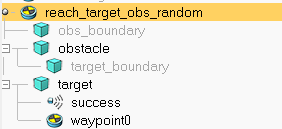
\includegraphics[scale=0.5]{assets/early-work/obs-random-scene-hierarchy.png}
    \caption{`ReachObs\_Random' Scene Hierarchy}
  \end{subfigure}
  \hfill
  \begin{subfigure}{0.45\linewidth}
    \centering
    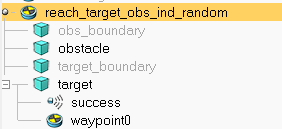
\includegraphics[scale=0.5]{assets/early-work/obs-ind-random-scene-hierarchy.png}
    \caption{`ReachObs\_IndRandom' Scene Hierarchy}
  \end{subfigure}
  \caption{Reaching Task with an Obstacle}\label{fig:reach-obs-random}
\end{figure}


\subsubsection{Wrist Camera Alone isn't Enough}

As expected, this is where the single wrist camera started showing its shortcomings. 

\todo{add graph of going around the obstacle but not quite reaching the target (wrist)}
\todo{show this with other combinations of cameras, comment on if the l/r without wrist can learn to go around the obstacle easily? maybe not, generalisation might be hard with no wrist}

The agent would easily move around the obstacle, however, would struggle to make the last steps in touching the target. This is mostly due to the fact that the demonstrations (which are provided by RLBench) are not necessarily pointing the wrist of the robot and hence the camera mounted there to look towards the target. This means that the wrist camera alone does not necessarily move towards the target, rather the robot learns to move behind the obstacle and nothing else.

From experiments I have realised that it learns to move around the obstacle easily, using simple behavioural cloning. However, getting the last nudge to actually reach the target is where it falls apart, especially in more realistic scenarios where the target is randomised behind the obstacle.

\subsubsection{Other Cameras}
Introducing the other cameras placed around in the environment, such as the \verb|left shoulder| or the \verb|right shoulder| cameras we can confirm that the wrist camera alone is not sufficient \todo{insert figure here with wrist vs others }, and the combination of wrist and other cameras are almost always the best as more coverage of the workspace guarantees less occlusions and more information the agent can work with to make decisions. It was clear that the wrist camera alone wasn't going to cut it unless it learnt to look towards the target.

\subsubsection{Implementing `Looking' into the Demonstrations}\todo{haven't done this yet}\label{ew-looking-at-target}
issues this is not easy might be working on this as a part of approach 2 later
Another solution might be to experiment with the demonstration system to make sure we are pointing the wrist camera (so, the hand of our robot) towards its target as a demonstration trajectory is calculated \todo{explain that this proved tricky and might not even be worth it}

If we can't implicitly encode the `looking' information through the demonstration that means we will have to inject this information into our agent some other way. Another way to make sure agent understands to look at the target is teaching it to actively seek out its target, either following previous works such as \todo{find some prior info tracking works add ref} where object priors are incorporated into the learning or with attention mechanisms that figure out what is important in a task without prior object information \todo{maybe reference this later}.  

\section{Expanding the Task Space: Grasping Tasks}
Another task which is likely to suffer from lack of viewpoints is a grasping task. So I designed these tasks around the idea of grasping. Firstly, a simple version (Figure \ref{fig:grasp-simple}) which the agent learns to reach then grasp the cubic target. 

Main differences between this and the reaching task is that the target here is tangible, so on top of being rendered it is also set to be \emph{collidable}. Another major addition is the usage of the \emph{extension string} as seen in \ref{subfig:simple-zoom-actions}, this instructs the demonstration engine to insert certain moves within the movement of the simple trajectory. In this case \verb|open_gipper()| ensures the gripper is open, then a later waypoint will instruct it to close.

\todo{maybe some experiment resutls here?}

The more complicated counterpart, shown in Figure \ref{fig:grasp-move}, is a scenario where the cube needs to be picked up then moved to the target location (designated in green)

\begin{figure}[htpb] % htpb allows all placement
  \centering
  \begin{subfigure}{0.3\linewidth}
    \centering
    \includegraphics[scale=0.2]{../fyp/assets/task-pics/grasp/simple-front.png}
    \caption{Front}\label{subfig:simple-front}
  \end{subfigure}
  \hfill
  \begin{subfigure}{0.5\linewidth}
    \centering
    \includegraphics[scale=0.3]{../fyp/assets/task-pics/grasp/simple-front-zoom-gripper_actions.png}
    \caption{Zoomed, with gripper action}\label{subfig:simple-zoom-actions}
  \end{subfigure}
  \caption{Simple Grasping Task}\label{fig:grasp-simple}
\end{figure}

\begin{figure}[htpb] % htpb allows all placement
  \centering
  \begin{subfigure}{0.45\linewidth}
    \centering
    \includegraphics[scale=0.2]{../fyp/assets/task-pics/grasp/move-front.png} 
    \caption{Front}\label{subfig:grasp-move-front}
  \end{subfigure}
  \hfill
  \begin{subfigure}{0.45\linewidth}
    \centering
    \includegraphics[scale=0.2]{../fyp/assets/task-pics/grasp/move-top.png}
    \caption{Top}\label{subfig:grasp-move-top}
  \end{subfigure}
  \caption{Grasping then moving}\label{fig:grasp-move}
\end{figure}


\missingfigure{grasp pic and possibly the demo gifs, }
\todo{add a picture with the cube grasped and the wrist camera view seen at that point}
Although, initially the wrist camera shouldn't pose any problems, as we advance through the task, especially after we have grasped something the wrist mounted camera becomes heavily obstructed and becomes unreliable so basing our decisions on this medium alone is not ideal.

\subsubsection{Observations}
What I got from these experiments was that the agent can benefit from understanding its surroundings at a higher level and more importantly remembering them. This is because once the camera becomes obstructed, as with \emph{Grasp Then Move}, even if the agent could do some exploration to find the target, it wouldn't be ideal due to the restricted view it has access to. So, observing the environment before, and remembering important parts will be vital for the later stages of tasks. I aim to explore some pre-policy visual exploration of the environment to be albeit to address issues such as this one.

\section{}